To measure the efficiency of the process of software development in GitHub first we focus on BMI, that was defined in section \ref{overview}. The chart below shows evolution of BMI pull requests by quarter, allowing us to check how pull requests are being managed by the community in the last quarter compared to previous quarters.

\begin{tabular}{p{9cm} p{5cm}}
	\vspace{0pt} 
	\hspace*{-6cm}  
	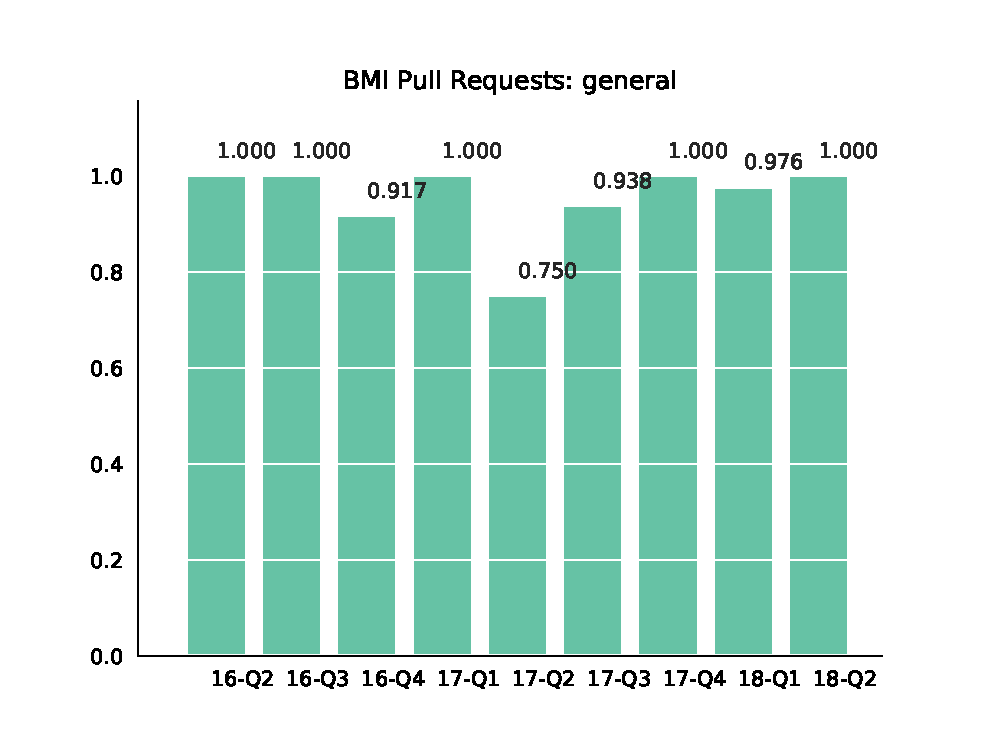
\includegraphics[scale=.75]{process/github_prs_bmipr.eps}
	& 
	\vspace{0pt}
	\begin{tabular}{l|l}%
		\bfseries Period & \bfseries Closed/Subm. % specify table head
		\csvreader[head to column names]{process/github_prs_bmipr.csv}{}% use head of csv as column names
		{\\\Date & \bmi}
	\end{tabular}
\end{tabular}

Besides, the next chart deals with timing. It shows the mean and median times to merge pull requests in GitHub (TTM, defined in section \ref{overview})--in days--for last quarter compared to previous ones.


\begin{tabular}{p{9cm} p{5cm}}
	\vspace{0pt} 
	\hspace*{-6cm}  
	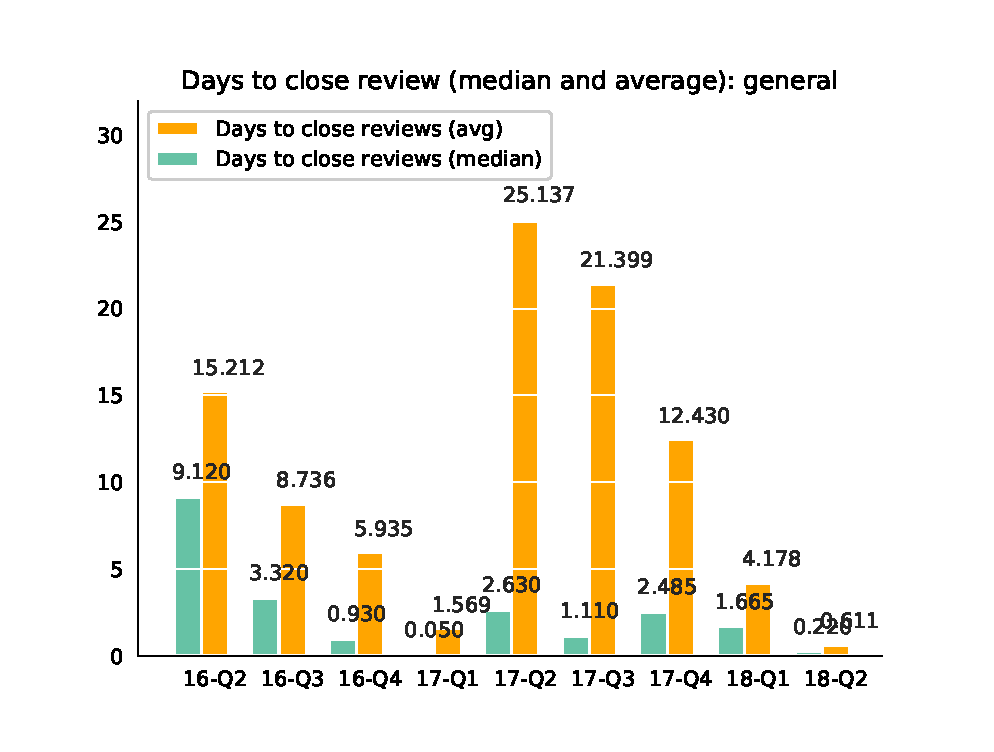
\includegraphics[scale=.75]{process/github_prs_days_to_close_pr_average_github_prs_days_to_close_pr_median.eps}
	& 
	\vspace{0pt}
	\begin{tabular}{l|r|r|}%
		\bfseries Period & \bfseries Median & \bfseries Mean % specify table head
		\csvreader[head to column names]{process/github_prs_days_to_close_pr_average_github_prs_days_to_close_pr_median.csv}{}% use head of csv as column names
		{\\\Date & \daystocloseprmedian & \daystoclosepraverage}
	\end{tabular}
\end{tabular}
